\documentclass[a4paper, 14pt]{extarticle}

\usepackage{../latexDependencies/misc/preamble2}

\geometry{a4paper}

% Название дисциплины
\newcommand{\subject}{Теория вероятности и математическая статистика} 

% Тип работы
% lab - для лабораторной работы 
% hw  - для домашней     работы
\newcommand{\task}{lab} 

% Номер работы
\newcommand{\taskNumber}{6} 

% Название работы
\newcommand{\taskNameOne}{Последовательный критерий} 
\newcommand{\taskNameTwo}{отношения правдоподобия} 

% Имя студента
\newcommand{\studentName}{Очкин Н.В.}

% Имя преподававателя
\newcommand{\teacherName}{Облакова Т.В.}

% Группа
\newcommand{\group}{ФН11-52Б}

% Вариант
\newcommand{\variant}{9}

\begin{document}

\graphicspath{ {../latexDependencies/images} } 
\normalsize

\newcommand{\printTask}{%
    \ifthenelse{\equal{\task}{lab}}{%
        лабораторной%
    }{%
        \ifthenelse{\equal{\task}{hw}}{%
            домашней%
        }{%
            Неизвестный тип задания%
        }%
    }%
}

\begin{titlepage}

    \begin{center}
        {\footnotesize \itshape Федеральное государственное бюджетное 
                       образовательное учреждение высшего образования}
    \end{center}

    \begin{minipage}[c]{0.1\textwidth}
        
\includegraphics[width=1.1\textwidth]{iconBMSTU}
    \end{minipage}
    \hfill
    \begin{minipage}[c]{0.9\textwidth}
        \centering
        \itshape
        \bfseries
        \small
        \guillemotleft Московский государственный технический университет \\
        имени Н.Э. Баумана\guillemotright \\
        (национальный исследовательский университет) \\
        (МГТУ им. Н.Э. Баумана) 
    \end{minipage}

    \vspace{0.5cm}
    \noindent\rule{\textwidth}{2pt} \\

    \noindent\uline{\textbf{ФАКУЛЬТЕТ} ФУНДАМЕНТАЛЬНЫЕ НАУКИ} \\
    \vspace{-5pt} \\
    \noindent\uline{\textbf{КАФЕДРА} ВЫЧИСЛИТЕЛЬНАЯ МАТЕМАТИКА И МАТЕМАТИЧЕСКАЯ} \\
    \vspace{-5pt} \\
    \noindent\uline{ФИЗИКА (ФН11)} \\
    \vspace{-5pt} \\
    \noindent\uline{\textbf{НАПРАВЛЕНИЕ ПОДГОТОВКИ} МАТЕМАТИКА И КОМПЬЮТЕРНЫЕ} \\
    \vspace{-5pt} \\
    \noindent\uline{НАУКИ (02.03.01)} \\

    \begin{center}
        \bfseries
        \textsc{О т ч е т} \\[10pt]
        по \printTask {} работе \textnumero {} \taskNumber
    \end{center}

    \vspace{10pt}

    \hspace{10pt} 
    \noindent \textbf{Название \printTask {} работы:} \par
    \vspace{5pt}
    \hspace{10pt} 
    \noindent \textbf{\uline{\taskNameOne}} \vspace{5pt} \\
    \null\hspace{31pt} 
    \textbf{\uline{\taskNameTwo}} \vspace{5pt} 

    \vspace{10pt}

    \begin{center}
        \bfseries
        Вариант \textnumero {} \variant
    \end{center}

    \vspace{20pt}

    \hspace{10pt} 
    \noindent \textbf{Дисциплина:} \par
    \vspace{10pt}
    \hspace{10pt} 
    \noindent {\large \subject}

    \vspace{10pt}

    \begin{flushright}
        \renewcommand{\arraystretch}{3}
        \begin{tabular}{r r r}
            \multicolumn{1}{l}{Студент группы \uline{\group}} & 
            $\quad \underset{\text{(Подпись, дата)}}{\underline{\hspace{3cm}}} \quad$ & 
            \multicolumn{1}{c}{$\underset{\text{(И.О. Фамилия)}}{\uline{\textbf{\studentName}}}$} \\

            \multicolumn{1}{l}{Преподаватель} & 
            $\quad \underset{\text{(Подпись, дата)}}{\underline{\hspace{3cm}}} \quad$ & 
            \multicolumn{1}{c}{$\underset{\text{(И.О. Фамилия)}}{\uline{\textbf{\teacherName}}}$} \\
        \end{tabular}
    \end{flushright}

    \vfill

    \begin{center}
        \small
        Москва, 2024
    \end{center}
\end{titlepage}


\newgeometry{left=25mm, right=25mm, top=20mm, bottom=20mm}

\graphicspath{ {../latexDependencies/images/LW6} }

% Customize section, subsection, subsubsection and paragraph styles
\titleformat{\section}
  {\normalfont\large\bfseries}{\thesection}{1em}{}

\titleformat{\subsection}
  {\normalfont\normalsize\bfseries}{\thesubsection}{1em}{}

\titleformat{\subsubsection}
  {\normalfont\small\bfseries}{\thesubsubsection}{1em}{}

\titleformat{\paragraph}
  {\small\small\bfseries}{\theparagraph}{1em}{}

\thispagestyle{empty}

\null\newpage

% \setcounter{tocdepth}{5}
% \setcounter{secnumdepth}{5}

% \pagenumbering{roman}

% \tableofcontents
% \newpage

\pagenumbering{arabic}
\setcounter{page}{1}

\setstretch{1}
\linespread{1.1}

\setlength{\parindent}{0pt}

\fontsize{12pt}{16pt}\selectfont

\definecolor{myblue}{HTML}{0A88C2}
\definecolor{myred}{HTML}{FF1B1C}
\definecolor{mygreen}{HTML}{386641}

\lstdefinestyle{mystyle}{
    basicstyle=\ttfamily\footnotesize,
    keywordstyle=\color{myblue},
    stringstyle=\color{myred},
    commentstyle=\color{green!50!black},
    showstringspaces=false,
    frame=leftline, 
    framesep=10pt, 
}

% Set the style for Python code
\lstset{style=mystyle, extendedchars=\true}

% --------------------------------------START--------------------------------------

\section*{Задание}\vspace{-20pt}\rule{\linewidth}{0.1mm}

\begin{enumerate}
    \item Постройте последовательный критерий Вальда для проверки гипотезы \( H_0: a = a_0 \) против альтернативы \( H_1: a = a_1 \) при известном \( \sigma = \sigma_1 \). Ошибка первого рода задана в условии, ошибка второго рода \( \beta \) вычислена вами в пункте 4.
    \item Примените построенный критерий к заданной выборке (порядок чтения - по столбцам), сформулируйте результат. Дайте графическую иллюстрацию последовательного критерия.
    \item Вычислите математическое ожидание момента принятия решения при основной гипотезе \( H_0 \) и при альтернативе \( H_1 \).
    \item Перепишите критерий \( S_1 \) из пункта 3 предыдущей задачи в виде \( \left( \frac{L(\vec{X_n}, a_1)}{L(\vec{X_n}, a_0)}  \geq C \right) \), отметьте на графике найденное значение и сравните результаты применения критериев Вальда и Неймана-Пирсона.
    \item Сформулируйте выводы.
\end{enumerate}

\section*{Исходные данные}\vspace{-20pt}\rule{\linewidth}{0.1mm}

\begin{center}
    \begin{tabular}{|c|c|c|c|c|c|c|c|c|}
        \hline
        $\alpha$ & $a_0$ & $\sigma_0$ & $a_1$ & $\sigma_1$ & $\varepsilon$ & $n$ & $\beta$ & $C_1$ \\
        \hline
        0.1      & 3      & 2.1       & 3.5   & 2.2        & 0.1           & 100 & 0.1608 & 3.2819 \\
        \hline
    \end{tabular}
\end{center}

\begin{equation*}
    \begin{vmatrix}
        -3.442 & 1.295 & 3.672 & 2.354 & 5.238 & 1.136 & 4.421 & 2.071 & 0.269 & 0.894 \\
        8.202 & 0.605 & -2.011 & 3.375 & 3.767 & 1.068 & 2.928 & -0.276 & 4.924 & 3.31 \\
        5.741 & 6.951 & 3.417 & 2.991 & 5.599 & 4.896 & 9.197 & 3.823 & 1.827 & 5.389 \\
        2.504 & 4.212 & -2.021 & 1.891 & 3.689 & 5.366 & 3.117 & 4.641 & 2.968 & 4.645 \\
        3.752 & 4.582 & 3.601 & 0.934 & 2.785 & 3.294 & 4.695 & 1.092 & 3.155 & 4.352 \\
        0.896 & 0.839 & 4.309 & 2.793 & 7.233 & 0.95 & 5.228 & 1.28 & 5.19 & 0.972 \\
        4.562 & 1.915 & 4.243 & 4.495 & 0.648 & 5.34 & 3.294 & 2.791 & 6.805 & 3.474 \\
        3.044 & 5.452 & 2.957 & 7.862 & 4.61 & 1.317 & 5.383 & 3.205 & -1.022 & 3.602 \\
        3.373 & 5.415 & 4.093 & 5.407 & 0.501 & 2.135 & 1.957 & 0.826 & 5.34 & 3.759 \\
        1.735 & -3.277 & 5.101 & 1.43 & 3.494 & 0.545 & 4.699 & 3.44 & 2.85 & 4.33 \\
    \end{vmatrix}
\end{equation*}

\newpage

\section*{Ход выполнения работы}\vspace{-20pt}\rule{\linewidth}{0.1mm}

Построим последовательный критерий Вальда для проверки гипотезы \\
$H_0: a = a_0 = 3$ против альтернативы $H_1: a = a_1 = 3.5$ при известном 
$\sigma = \sigma_1 = 2.2$.\\

Найдем такие границы $A$ и $B$, которые удовлетворяют следующему условию:

\begin{equation*}
    B < z(\vec{X_n}) < A,
\end{equation*}

где 

\begin{equation*}
    z(\vec{X_n}) = \cfrac{L(\vec{X_n}, a_1)}{L(\vec{X_n}, a_0)} \qquad - \qquad \text{функция отношения правдоподобия}
\end{equation*}

Положим 

\begin{equation*}
    \nu = \text{min}\left\{ n: z\left( \vec{X_n} \right) \notin (B, A) \right\},
\end{equation*}

\vspace{10pt}

то есть статистикой критерия будет $z(\nu, X_1, ..., X_\nu)$.\\

Сформулируем критерий Вальда:
\begin{itemize}
    \item[--] если $z\left( \vec{X_n} \right) \geq A$, то принимается $H_1$ 
    \item[--] если $z\left( \vec{X_n} \right) \leq B$, то принимается $H_0$ 
\end{itemize}

\vspace{10pt}

Тогда ошибка первого рода принимает вид:

\begin{equation*}
    \alpha = P \left( z\left( \vec{X_n} \right) \geq A | H_0 \right),
\end{equation*}

а ошибка второго рода:

\begin{equation*}
    \beta = P \left( z\left( \vec{X_n} \right) \leq B | H_1 \right).
\end{equation*}

\vspace{10pt}

Постоянные $A$ и $B$ вычислим по формулам Вальда:

\begin{equation*}
    A = \cfrac{1 - \beta}{\alpha} \qquad B = \cfrac{\beta}{1 - \alpha}
\end{equation*}

\begin{center}
  \begin{lstlisting}[language=Python]
A_ = (1 - beta)/alpha
B_ = beta/(1 - alpha)
  \end{lstlisting}
\end{center}

\vspace{-20pt}

\begin{equation*}
    A \approx 8.392 \qquad B \approx 0.1787
\end{equation*}

\newpage

Вычислим отношение правдоподобия:

\begin{gather*}
    \cfrac{L(\vec{X_n}, a_1, \sigma_1)}{L(\vec{X_n}, a_0, \sigma_1)} \hspace{10pt}=\hspace{10pt} 
    \prod_{i=1}^{n} \cfrac{p(X_i, a_1, \sigma_1)}{p(X_i, a_0, \sigma_1)} \hspace{10pt}=\hspace{10pt}
    \cfrac{\prod\limits_{i=1}^n \cfrac{1}{\sigma_1\sqrt{2\pi}} 
    \cdot e^{\cfrac{-(X_i-a_1)^2}{2\sigma^2_1}}}{\prod\limits_{i=1}^n 
    \cfrac{1}{\sigma_1\sqrt{2\pi}} \cdot e^{\cfrac{-(X_i-a_0)^2}{2\sigma^2_1}}} \hspace{10pt} = \\[2em]
    = \hspace{10pt} \prod\limits_{i=1}^n \exp \left[ \cfrac{-(X_i-a_1)^2}{2\sigma^2_1} + 
    \cfrac{(X_i-a_0)^2}{2\sigma^2_1} \right] \hspace{10pt} = \hspace{10pt} 
    \exp \left[\sum\limits_{i=1}^n\cfrac{-(X_i-a_1)^2 + (X_i-a_0)^2}{2\sigma^2_1} \right] \hspace{10pt} = \\[2em]
    = \hspace{10pt} \exp \left[ n \cdot \cfrac{a^2_0 - a^2_1}{2\sigma^2_1} + \cfrac{a_1 - a_0}{\sigma^2_1} 
    \cdot \sum_{i=1}^n X_i \right]
\end{gather*}

Применим построенный критерий к данной выборке. \\
Введем следующее обозначение:

\begin{equation*}
    z = X^T
\end{equation*}

Тогда

\begin{equation*}
    Z(j) = \prod_{i=1}^j \exp \left[ \cfrac{a^2_0 - a^2_1}{2\sigma^2_1} + 
    \cfrac{a_1 - a_0}{\sigma^2_1} z_i \right]
\end{equation*}

Приведем графическую иллюстрацию последовательного критерия: 

\begin{center}
  \begin{lstlisting}[language=Python]
def Z(j):
    res = 1
    for i in range(0, j + 1):
        res *= np.exp((a0**2 - a1**2)/(2*sigma1**2) + \
                      (a1 - a0)/sigma1**2 * data_[i])
    return res
  \end{lstlisting}
\end{center}

\vfill

\begin{equation*}
    \scalebox{1.5}{
        $\downarrow$
    }
\end{equation*}

\vfill\newpage

\begin{center}
    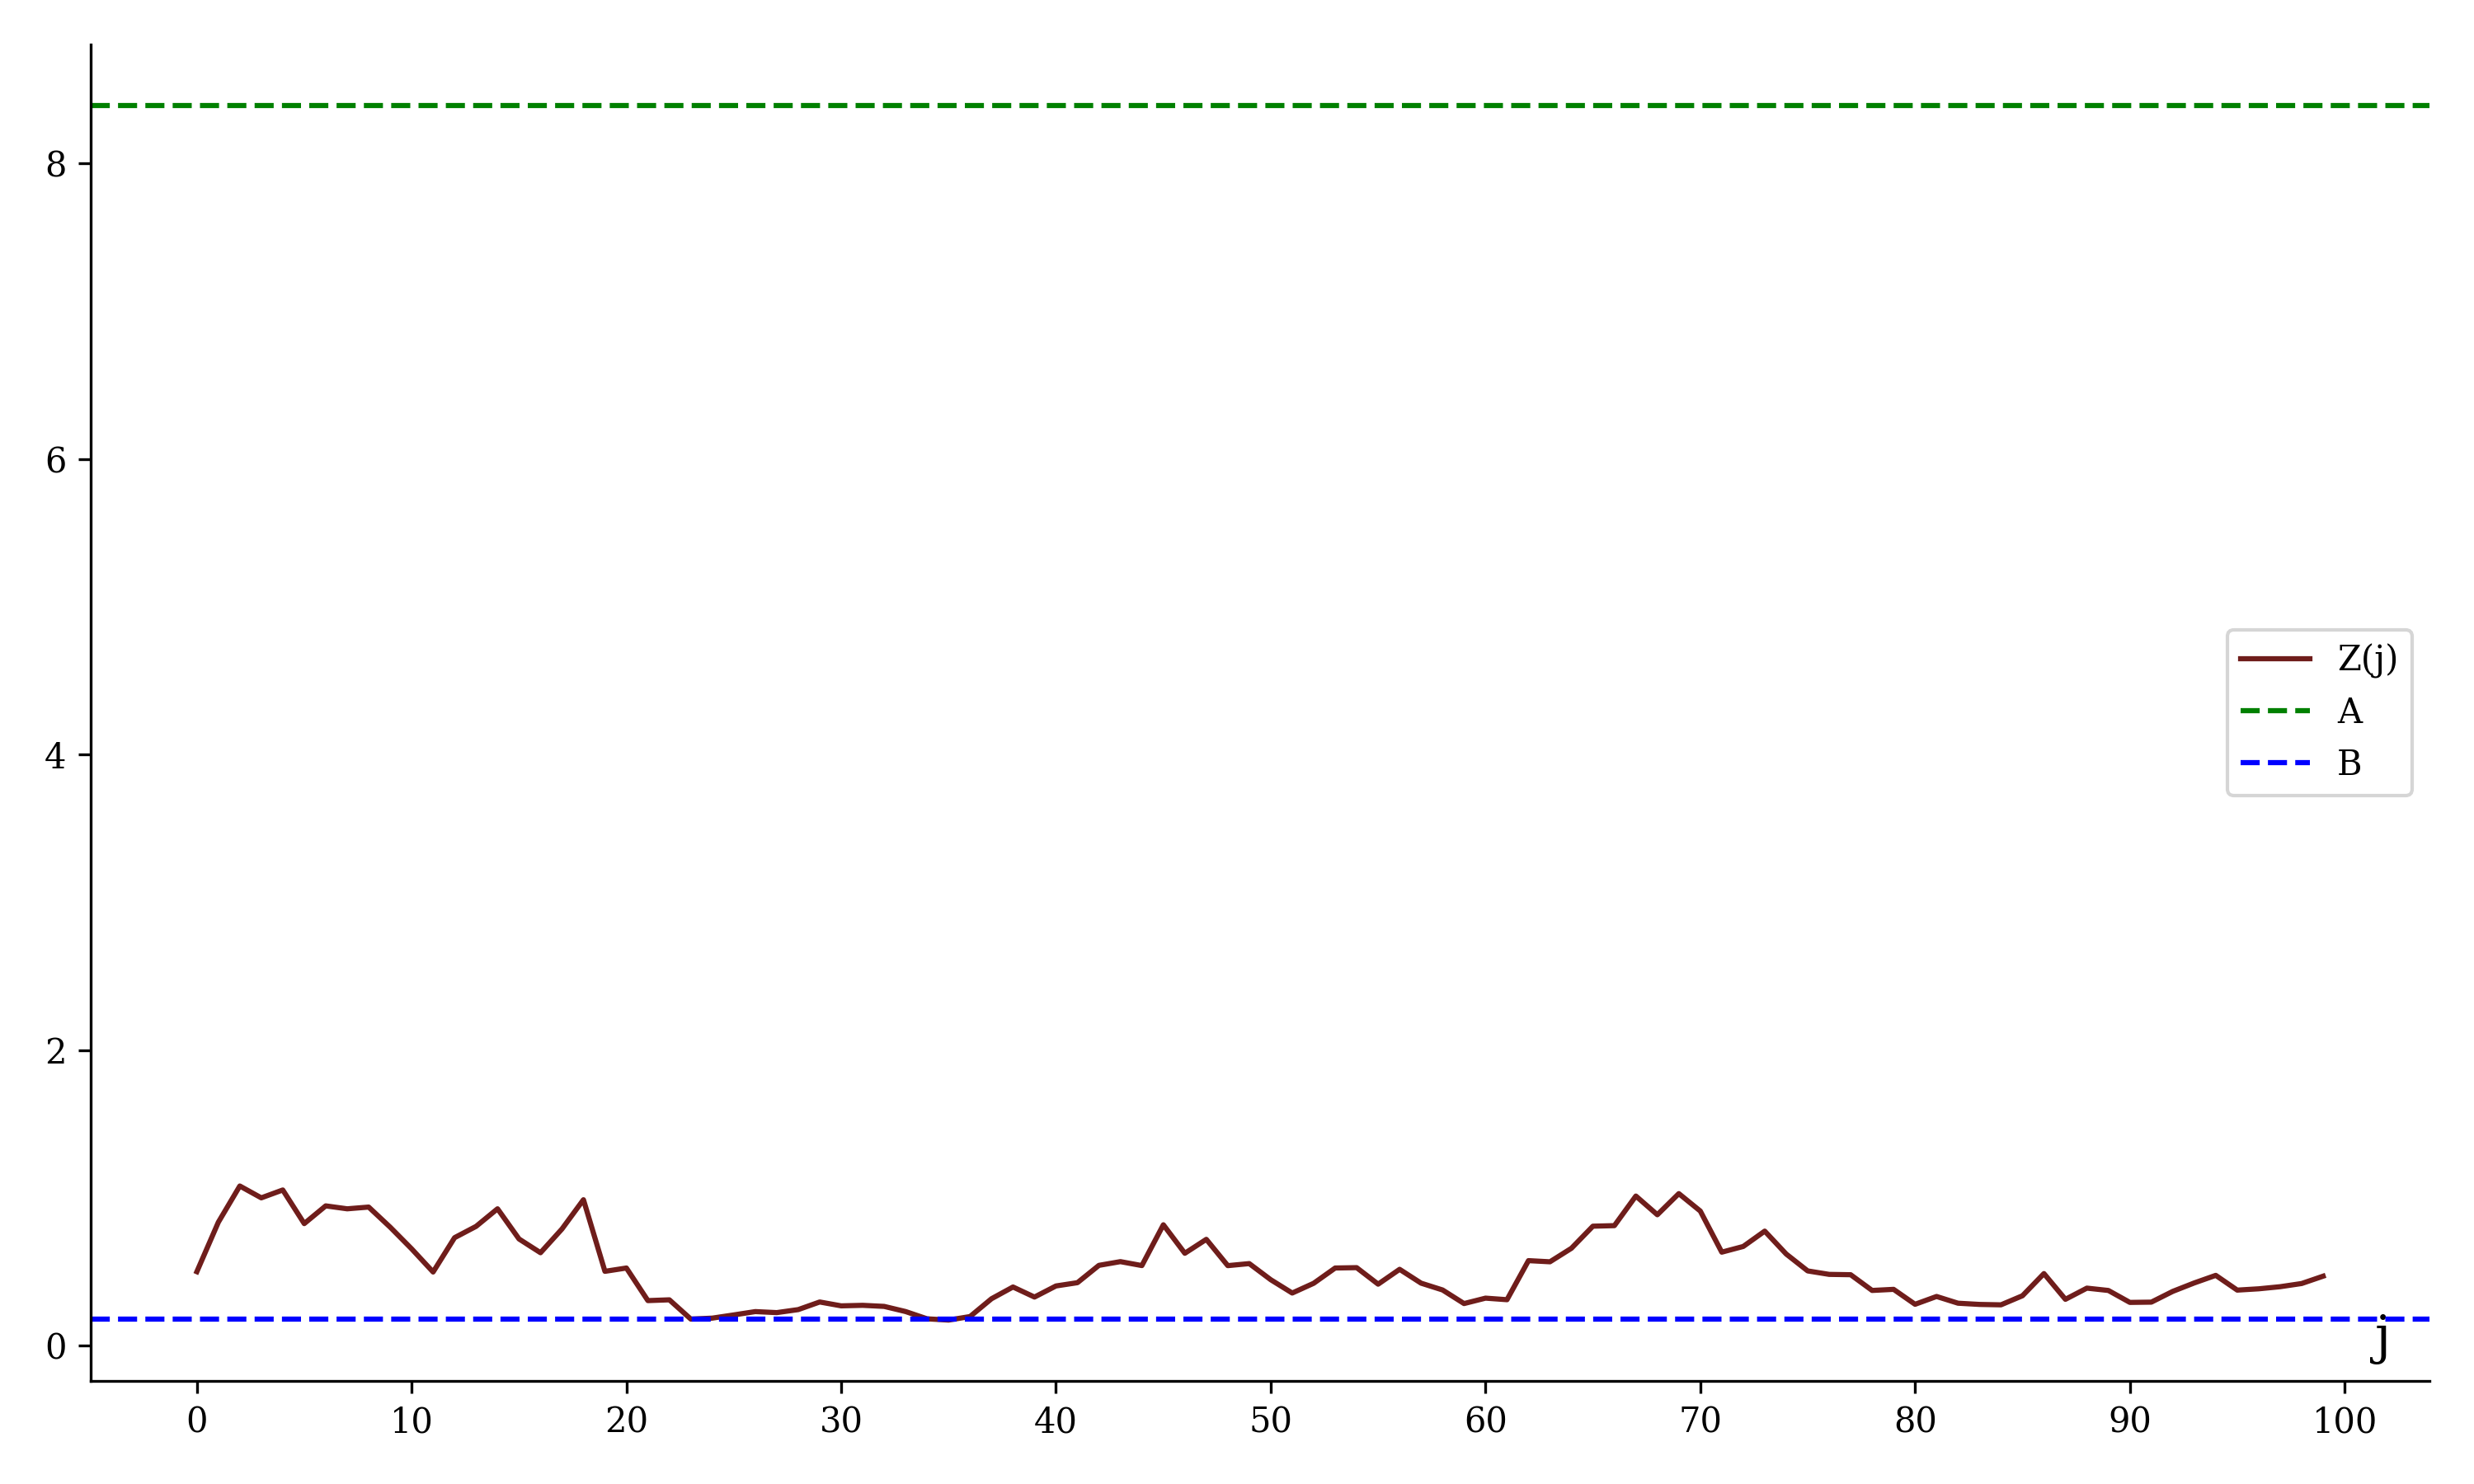
\includegraphics[width=\textwidth, height=\textheight, keepaspectratio]{iterative_crit_A_B} \\
\end{center}

Заметим, что график пересекает прямую B $\Rightarrow$ принимается гипотеза $H_0$.\\

Вычислим математическое ожидание момента принятия решения при основной гипотезе 
$H_0: a = a_0 = 3$ и при альтернативе $H_1: a = a_1 = 3.5$.\\

Найдем математическое ожидание момента принятия решения при основной гипотезе $H_0$:

\begin{equation*}
    M_{a_0}\nu = \cfrac{\alpha ln(A) + (1 - \alpha)ln(B)}{M_0}
\end{equation*}

\begin{equation*}
    M_0 = M_{a_0}ln\left(\cfrac{\rho(X_k, a_1, \sigma_1)}{\rho(X_k, a_0, \sigma_1)}\right) = 
    \cfrac{-(a_1 - a_0)^2}{2\sigma^2_1}
\end{equation*}

\begin{center}
  \begin{lstlisting}[language=Python]
M0_ = -(a1 - a0)**2/(2 * sigma1**2)
Ma0nu_ = (alpha * np.log(A_) + (1 - alpha) * np.log(B_))/M0_
  \end{lstlisting}
\end{center}

\vspace{-10pt}

\begin{equation*}
    M_0 \approx -0.025826 \qquad M_{a_0}\nu \approx 51.779566
\end{equation*}

\newpage

Найдем математическое ожидание момента принятия решения при основной гипотезе $H_1$:

\begin{equation*}
    M_{a_1}\nu = \cfrac{\beta ln(B) + (1 - \beta)ln(A)}{M_1}
\end{equation*}

\begin{equation*}
    M_1 = M_{a_1}ln\left(\cfrac{\rho(X_k, a_1, \sigma_1)}{\rho(X_k, a_0, \sigma_1)}\right) = 
    \cfrac{(a_1 - a_0)^2}{2\sigma^2_1}
\end{equation*}

\begin{center}
  \begin{lstlisting}[language=Python]
M1_ = (a1 - a0)**2/(2 * sigma1**2)
Ma1nu_ = (beta * np.log(B_) + (1 - beta) * np.log(A_))/M1_
  \end{lstlisting}
\end{center}

\vspace{-10pt}

\begin{equation*}
    M_1 \approx 0.0258264 \qquad M_{a_1}\nu \approx 58.400497
\end{equation*}

\vspace{10pt}

Перепишем критическое множество из пункта 3 в виде 
\( \left( \frac{L(\vec{X_n}, a_1)}{L(\vec{X_n}, a_0)}  \geq C \right) \), 
отметим на графике и сравним результаты применения критериев Вальда и Неймана-Пирсона.\\

Запишем критическое множество в следующем виде: 

\begin{equation*}
    S = \left\{\cfrac{L(X_k, a_1, \sigma_1)}{L(X_k, a_0, \sigma_1)} \geq C\right\} = 
    \left\{\exp\left[n \cdot \cfrac{a^2_0 - a^2_1}{2\sigma^2_1} + \cfrac{a_1 - a_0}{\sigma^2_1} 
    \cdot \sum\limits_{i=1}^n X_i\right] \geq C\right\}
\end{equation*}

\vspace{10pt}

Выразим $\overline{X}$:

\vspace{-20pt}

\begin{equation*}
    S = \left\{n \cfrac{a^2_0 - a^2_1}{2\sigma^2_1} + 
    \cfrac{a_1 - a_0}{\sigma^2_1} \sum\limits_{i=1}^n X_i \geq ln(C)\right\} = 
    \left\{\cfrac{1}{n} \sum\limits_{i=1}^n X_i \geq \cfrac{\left(\cfrac{ln(C)}{n} - 
     \cfrac{a^2_0 - a^2_1}{2\sigma^2_1}\right) \sigma^2_1}{(a_1 - a_0)}\right\}
\end{equation*}

Заметим, что $a_1 - a_0 = 0.5 > 0 \Rightarrow$ при делении знак неравенства не меняется. \\

Следовательно:

\begin{equation*}
    C_1 = 3.2819 = \cfrac{\left(\cfrac{ln(C)}{n} - \cfrac{a^2_0 - a^2_1}{2\sigma^2_1}\right) \sigma^2_1}{(a_1 - a_0)}
\end{equation*}

Итого:

\begin{equation*}
    C = \exp \left[ \cfrac{C_1 (a_1 - a_0) n}{\sigma_1^2} + 
    n \cfrac{a_0^2 - a_1^2}{2 \sigma_1^2} \right]
\end{equation*}

\begin{center}
  \begin{lstlisting}[language=Python]
C_ = np.exp((C1 * (a1 - a0) * n) / (sigma1**2) + \
                            n * (a0**2 - a1**2)/(2 * sigma1**2))
  \end{lstlisting}
\end{center}

\vspace{-10pt}

\begin{equation*}
    C \approx 1.39034
\end{equation*}

\vspace{10pt}

Таким образом, получаем критическое множество:

\begin{equation*}
    S = \left\{\cfrac{L(X_k, a_1, \sigma_1)}{L(X_k, a_0, \sigma_1)} \geq 1.39034\right\}
\end{equation*}

\vspace{10pt}

Приведем графическую иллюстрацию последовательного критерия: 

\begin{center}
    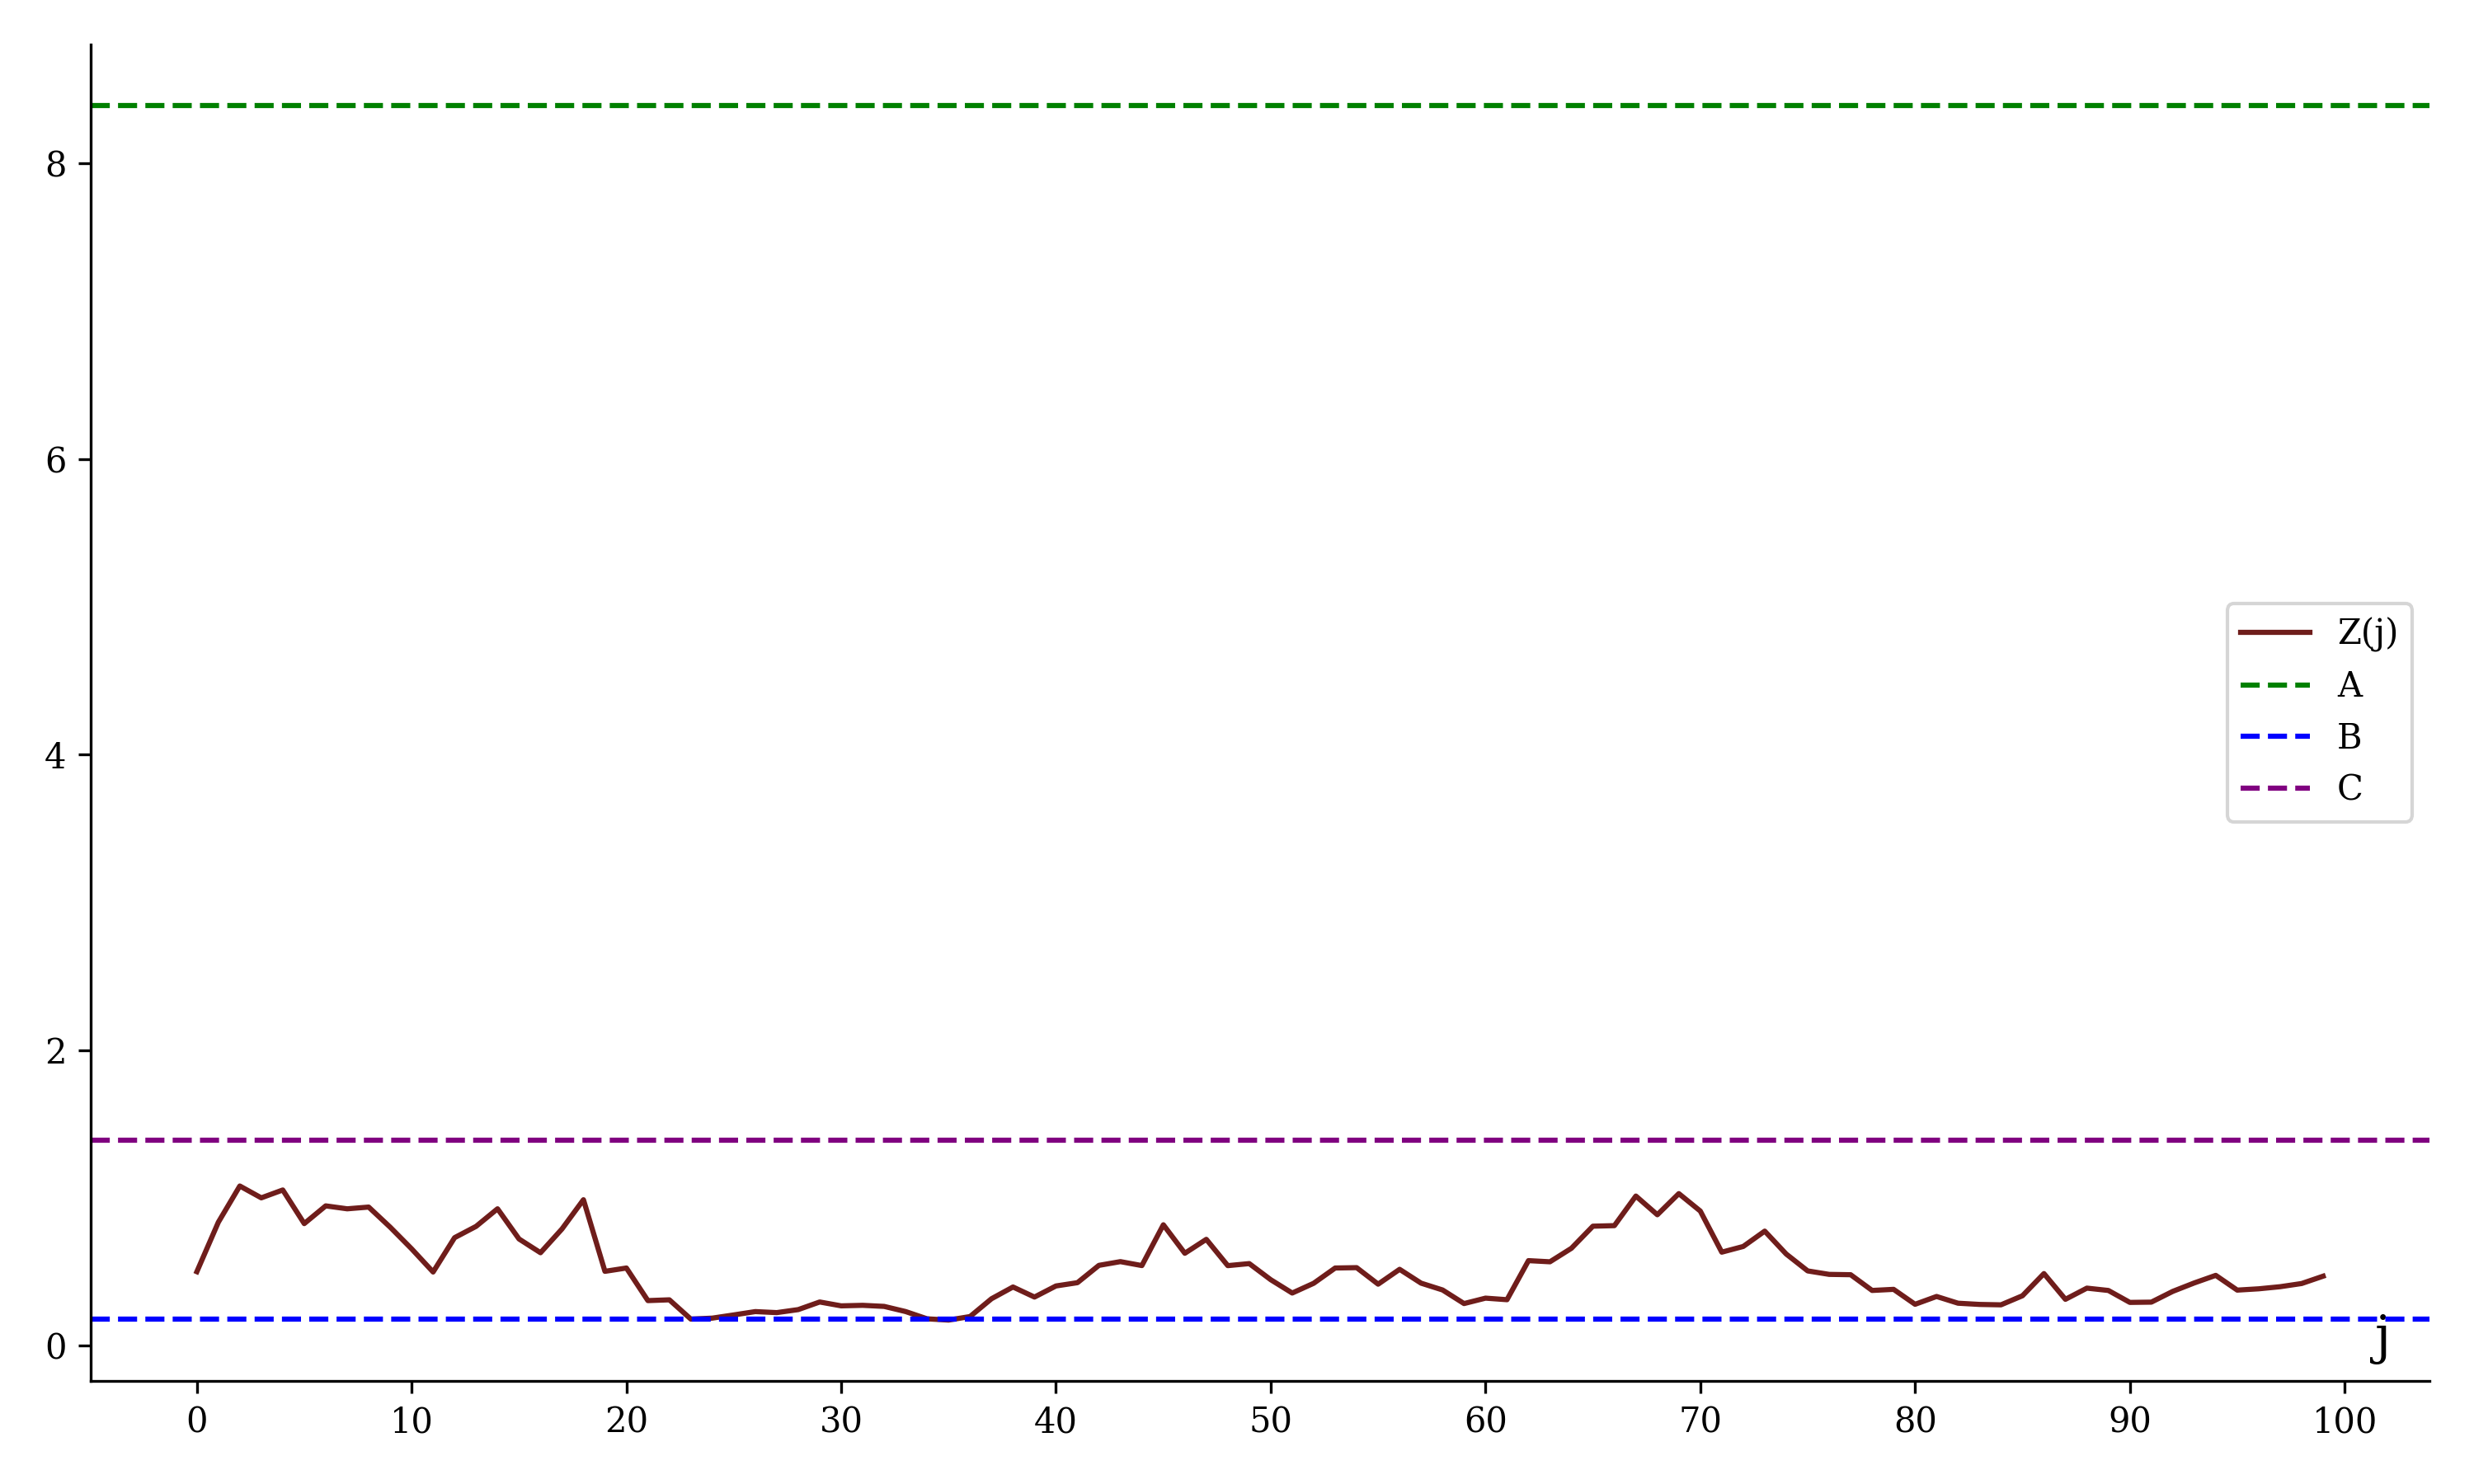
\includegraphics[width=\textwidth, height=\textheight, keepaspectratio]{iterative_crit_A_B_C} \\
\end{center}

При $n = 100$:

\begin{center}
  \begin{lstlisting}[language=Python]
    likelihoodRatio_ = np.exp(n * (a0**2 - a1**2)/(2 * sigma1**2) + \
                                    (a1 - a0)/sigma1**2 * np.sum(data_))
  \end{lstlisting}
\end{center}

\vspace{-20pt}

\begin{equation*}
    \frac{L(\bar{X}_n, a_1, \sigma_1)}{L(\bar{X}_n, a_0, \sigma_1)} \approx 0.47066 < C
\end{equation*}

\vspace{10pt}

$\Rightarrow$ принимается гипотеза $H_0$.

\newpage

\section*{Вывод}\vspace{-20pt}\rule{\linewidth}{0.1mm}

В процессе выполнения задания мы научились строить последовательный критерий Вальда 
для проверки простых гипотез о среднем значении нормального закона 
(основная гипотеза $H_0: a=a_0$  против альтернативы $H_1:a=a_1$ при известном 
$\sigma=\sigma_1$) а также применять построенный критерий к заданной выборке, 
вычислять математическое ожидание момента принятия решения при основной гипотезе $H_0$ 
и при альтернативе $H_1$. Было установлено, что критерий Вальда и критерий Неймана-Пирсона 
дали одинаковый результат.

\newpage

\section*{Приложение}\vspace{-20pt}\rule{\linewidth}{0.1mm}

Программный код, с помощью которого была выполнена данная лабораторная работа.\\

\begin{center}
  \begin{lstlisting}[language=Python]
import numpy as np
from IPython.display import Math, display
import matplotlib.pyplot as plt

data_ = np.array([
    [-3.442, 1.295, 3.672, 2.354, 5.238, 1.136, 4.421, 2.071, 0.269, 0.894],
    [8.202, 0.605, -2.011, 3.375, 3.767, 1.068, 2.928, -0.276, 4.924, 3.31],
    [5.741, 6.951, 3.417, 2.991, 5.599, 4.896, 9.197, 3.823, 1.827, 5.389],
    [2.504, 4.212, -2.021, 1.891, 3.689, 5.366, 3.117, 4.641, 2.968, 4.645],
    [3.752, 4.582, 3.601, 0.934, 2.785, 3.294, 4.695, 1.092, 3.155, 4.352],
    [0.896, 0.839, 4.309, 2.793, 7.233, 0.95, 5.228, 1.28, 5.19, 0.972],
    [4.562, 1.915, 4.243, 4.495, 0.648, 5.34, 3.294, 2.791, 6.805, 3.474],
    [3.044, 5.452, 2.957, 7.862, 4.61, 1.317, 5.383, 3.205, -1.022, 3.602],
    [3.373, 5.415, 4.093, 5.407, 0.501, 2.135, 1.957, 0.826, 5.34, 3.759],
    [1.735, -3.277, 5.101, 1.43, 3.494, 0.545, 4.699, 3.44, 2.85, 4.33]
])

data_ = data_.T
new_data_ = []

for i in range(len(data_)):
    for j in range(len(data_[i])):
        new_data_.append(data_[i][j])

data_ = new_data_
data_

alpha = 0.1
a0 = 3
sigma0 = 2.1
a1 = 3.5
sigma1 = 2.2
epsilon = 0.1
n = 100
beta = 0.1608
C1 = 3.2819

def decorate_plot(ax, x_ticks, xname, yname, loc=(-0.025, -0.3)):
    SIZE_TICKS = 10

    # Eliminate upper and right axes
    ax.spines['right'].set_color('none')
    ax.spines['top'].set_color('none')

    # Show ticks in the left and lower axes only
    ax.xaxis.set_ticks_position('bottom')
    ax.yaxis.set_ticks_position('left')

    # axis names
    ax.set_xlabel(xname, fontsize=15)
    ax.xaxis.set_label_coords(0.98, 0.05)

    ax.set_ylabel(yname, rotation=0, fontsize=15)
    ax.yaxis.set_label_coords(0.025, 0.95)

    ax.set_xticks(x_ticks)

    # Adjust the font size of the tick labels
    ax.tick_params(axis='both', which='major', labelsize=SIZE_TICKS)

    plt.legend(fontsize=10, loc=loc)

    # Update font settings
    plt.rcParams.update({'font.family': 'serif', 'font.size': 12})

    # Adjust layout
    plt.tight_layout()

A_ = (1 - beta)/alpha
B_ = beta/(1 - alpha)

print(f'A: {A_}')
print(f'B: {B_}')

def Z(j):
    res = 1
    for i in range(0, j + 1):
        res *= np.exp((a0**2 - a1**2)/(2*sigma1**2) + (a1 - a0)/sigma1**2 * data_[i])
    return res

def buildBar(filename):
    RED = '#6F1D1B'

    _, ax = plt.subplots(figsize=(10, 6))

    x_values = np.arange(0, n)
    y_values = [Z(int(x)) for x in x_values]

    ax.plot(x_values, 
           y_values, 
           color=RED, 
           linestyle='-', 
           linewidth=1.5,
           label='Z(j)')
    
    ax.axhline(y=A_, color='green', linestyle='--', label=f'A')
    ax.axhline(y=B_, color='blue', linestyle='--', label=f'B')

    decorate_plot(ax, np.arange(0,n + 10,10), 'j', '', loc='best')

    # plt.savefig(f'{filename}.png', dpi=300, transparent=True)

    plt.show()

buildBar('iterative_crit_A_B')

M0_ = -(a1 - a0)**2/(2 * sigma1**2)
Ma0nu_ = (alpha * np.log(A_) + (1 - alpha) * np.log(B_))/M0_

display(Math(f'$M_0 = {M0_}$'))
display(Math(f'$M_{{a_0}}\\nu = {Ma0nu_}$'))

M1_ = (a1 - a0)**2/(2 * sigma1**2)
Ma1nu_ = (beta * np.log(B_) + (1 - beta) * np.log(A_))/M1_

display(Math(f'$M_1 = {M1_}$'))
display(Math(f'$M_{{a_1}}\\nu = {Ma1nu_}$'))

a1 - a0

C_ = np.exp((C1 * (a1 - a0) * n) / (sigma1**2) + n * (a0**2 - a1**2)/(2 * sigma1**2))

print(f'C = {C_}')

def buildBar(filename):
    RED = '#6F1D1B'

    _, ax = plt.subplots(figsize=(10, 6))

    x_values = np.arange(0, n)
    y_values = [Z(int(x)) for x in x_values]

    ax.plot(x_values, 
           y_values, 
           color=RED, 
           linestyle='-', 
           linewidth=1.5,
           label='Z(j)')
    
    ax.axhline(y=A_, color='green', linestyle='--', label=f'A')
    ax.axhline(y=B_, color='blue', linestyle='--', label=f'B')
    ax.axhline(y=C_, color='purple', linestyle='--', label=f'C')

    decorate_plot(ax, np.arange(0,n + 10,10), 'j', '', loc='best')

    # plt.savefig(f'{filename}.png', dpi=300, transparent=True)

    plt.show()

buildBar('iterative_crit_A_B_C')

likelihoodRatio_ = np.exp(n * (a0**2 - a1**2)/(2 * sigma1**2) + (a1 - a0)/sigma1**2 * np.sum(data_))
display(Math(f'$$\\frac{{L(\\bar{{X}}_n, a_1, \\sigma_1)}}{{L(\\bar{{X}}_n, a_0, \\sigma_1)}} = {likelihoodRatio_}$$'))
  \end{lstlisting}
\end{center}

\end{document}
